\documentclass{article}[18pt]
\ProvidesPackage{format}
%Page setup
\usepackage[utf8]{inputenc}
\usepackage[margin=0.7in]{geometry}
\usepackage{parselines} 
\usepackage[english]{babel}
\usepackage{fancyhdr}
\usepackage{titlesec}
\hyphenpenalty=10000

\pagestyle{fancy}
\fancyhf{}
\rhead{Sam Robbins}
\rfoot{Page \thepage}

%Characters
\usepackage{amsmath}
\usepackage{amssymb}
\usepackage{gensymb}
\newcommand{\R}{\mathbb{R}}

%Diagrams
\usepackage{pgfplots}
\usepackage{graphicx}
\usepackage{tabularx}
\usepackage{relsize}
\pgfplotsset{width=10cm,compat=1.9}
\usepackage{float}

%Length Setting
\titlespacing\section{0pt}{14pt plus 4pt minus 2pt}{0pt plus 2pt minus 2pt}
\newlength\tindent
\setlength{\tindent}{\parindent}
\setlength{\parindent}{0pt}
\renewcommand{\indent}{\hspace*{\tindent}}

%Programming Font
\usepackage{courier}
\usepackage{listings}
\usepackage{pxfonts}

%Lists
\usepackage{enumerate}
\usepackage{enumitem}

% Networks Macro
\usepackage{tikz}


% Commands for files converted using pandoc
\providecommand{\tightlist}{%
	\setlength{\itemsep}{0pt}\setlength{\parskip}{0pt}}
\usepackage{hyperref}

% Get nice commands for floor and ceil
\usepackage{mathtools}
\DeclarePairedDelimiter{\ceil}{\lceil}{\rceil}
\DeclarePairedDelimiter{\floor}{\lfloor}{\rfloor}

% Allow itemize to go up to 20 levels deep (just change the number if you need more you madman)
\usepackage{enumitem}
\setlistdepth{20}
\renewlist{itemize}{itemize}{20}

% initially, use dots for all levels
\setlist[itemize]{label=$\cdot$}

% customize the first 3 levels
\setlist[itemize,1]{label=\textbullet}
\setlist[itemize,2]{label=--}
\setlist[itemize,3]{label=*}

% Definition and Important Stuff
% Important stuff
\usepackage[framemethod=TikZ]{mdframed}

\newcounter{theo}[section]\setcounter{theo}{0}
\renewcommand{\thetheo}{\arabic{section}.\arabic{theo}}
\newenvironment{important}[1][]{%
	\refstepcounter{theo}%
	\ifstrempty{#1}%
	{\mdfsetup{%
			frametitle={%
				\tikz[baseline=(current bounding box.east),outer sep=0pt]
				\node[anchor=east,rectangle,fill=red!50]
				{\strut Important};}}
	}%
	{\mdfsetup{%
			frametitle={%
				\tikz[baseline=(current bounding box.east),outer sep=0pt]
				\node[anchor=east,rectangle,fill=red!50]
				{\strut Important:~#1};}}%
	}%
	\mdfsetup{innertopmargin=10pt,linecolor=red!50,%
		linewidth=2pt,topline=true,%
		frametitleaboveskip=\dimexpr-\ht\strutbox\relax
	}
	\begin{mdframed}[]\relax%
		\centering
		}{\end{mdframed}}



\newcounter{lem}[section]\setcounter{lem}{0}
\renewcommand{\thelem}{\arabic{section}.\arabic{lem}}
\newenvironment{defin}[1][]{%
	\refstepcounter{lem}%
	\ifstrempty{#1}%
	{\mdfsetup{%
			frametitle={%
				\tikz[baseline=(current bounding box.east),outer sep=0pt]
				\node[anchor=east,rectangle,fill=blue!20]
				{\strut Definition};}}
	}%
	{\mdfsetup{%
			frametitle={%
				\tikz[baseline=(current bounding box.east),outer sep=0pt]
				\node[anchor=east,rectangle,fill=blue!20]
				{\strut Definition:~#1};}}%
	}%
	\mdfsetup{innertopmargin=10pt,linecolor=blue!20,%
		linewidth=2pt,topline=true,%
		frametitleaboveskip=\dimexpr-\ht\strutbox\relax
	}
	\begin{mdframed}[]\relax%
		\centering
		}{\end{mdframed}}
\lhead{MCS - DMLA - Term 2}


\begin{document}
\begin{center}
\underline{\huge Modular Arithmetic}
\end{center}
\section{Basic modular arithmetic}
\subsection{Definition}
if a,b are integers and m is a positive integer then a is congruent to b modulo m iff m|(a-b). Notation $a\equiv b (mod m)$\\
Example: 8$\equiv 5 ( \bmod 3 )$ because 3$| ( 8 - 5 ) ; - 5 \equiv 9 ( \bmod 7 )$ because 7$| ( - 5 - 9 )$
\subsection{Lemma}
If a,b,m are integers and $m>0$ then $a\equiv b (mod m)$ iff $rem(a,m)=rem(b,m)$
\subsection{Lemma}
Let m be a positive integer and let $a\equiv b (mod m)$ and $c\equiv d (mod m)$ Then
$$a + c \equiv b + d ( \bmod m ) \quad \text { and } \quad a c \equiv b d ( \bmod m )$$
\section{Linear congruences}
Congruences work a lot like equations, but there are some differences:
\begin{itemize}
	\item if $ac\equiv bc (\bmod m)$ and $c \not\equiv 0 (\bmod m)$ it is possible that $a\not\equiv b (\bmod m)$. For example  $2 \cdot 3 \equiv 4 \cdot 3 ( \bmod 6 ) ,$ but $2 \neq 4 ( \bmod 6 )$
	\item If $a\equiv b (\bmod m)$ and $c\equiv d (\bmod m)$, it is possible that $a^c\not\equiv d^d (\bmod m)$
	\item A congruence of the form $ax\equiv b(\bmod m)$ is called a \textbf{linear congruence}
	\item Such congruences often appear in applications of number theory
	\item Solving such a congruence means finding all c (by default, in the range $\{0,1,...,m-1\}$) such that $ac\equiv b (\bmod m)$, such c might not be unique
\end{itemize}
\subsection{Example}
Solve $3x+1 \equiv 5 (\bmod 7)$\\
Subtract 1 from both sides, get $3x\equiv 4(\bmod 7)$\\
Now multiply both sides by 5, have $15x=20 (\bmod 7)$\\
Since 15$\equiv 1 ( \bmod 7 )$ and $20 \equiv 6 ( \bmod 7 ) ,$ have $x \equiv 6 ( \bmod 7 ) .$ So $x = 6$
\section{Multiplicative inverses}
\begin{itemize}
	\item An easy way to solve equation $ax=b$ is to multiply both parts by $a^{-1}$
	\item We cannot do this within integers, but we often can when working modulo m
	\item Call $\overline{a}$ the (multiplicative) inverse of a modulo m if $\overline { \mathbf { a } } a \equiv 1 ( \bmod m )$
	\item Multiplicative inverses do not always exist, e.g. $2\overline{a}\not\equiv 1 (\bmod 4)$ for any $\overline{a}$
\end{itemize}
\subsection{Theorem}
If gcd(a,m)=1 then the inverse of a modulo m exists, and is unique (that is, there is a unique $0\leqslant\overline{a}<m$ with $\overline{a}a\equiv 1 (\bmod m)$)
\subsection{Proof}
We show existence, and leave uniqueness as an exercise\\
Since gcd(a,m)=1, we have sa+tm=1 for some $s,t$. Then $sa\equiv 1 (\bmod m)$\\
Let $s=qm+r$ where $0\leqslant r <m$, then $ra=(s-qm)a\equiv sa \equiv 1 (\bmod m)$ so r is the required inverse
\begin{itemize}
	\item note that s can be found by using euclid's algorithm. Then $r$ is easy to find
\end{itemize}
\section{The Chinese remainder theorem}
\subsection{Theorem}
Let $m_1,...,m_n$ be pairwise relatively prime positive integers and $a_1,...,a_n$ arbitrary integers. Then the system
$$\begin{aligned} x & \equiv a _ { 1 } \left( \bmod m _ { 1 } \right) \\ x & \equiv a _ { 2 } \left( \bmod m _ { 2 } \right) \\ & \vdots \\ x & \equiv a _ { n } \left( \bmod m _ { n } \right) \end{aligned}$$
has a unique solution modulo $m=m_1m_2\cdots m_n$. That is, there is a unique solution x with $-\leqslant x <m$ and every other solution is congruent to x modulo m.
\subsection{Proof}
Let $M_k=m/m_k$\\
We have $gcd(M_k,m_k)$. Hence $M_ky_k\equiv q (\bmod m_k)$ for some $y_k$\\
Let $x=a_1M_1y_1+a_2M_2y_2+...+a_nM_ny_n$\\
We show that $x\equiv a_k (\bmod m_k)$ for all k.\\
Notice that $M_j\equiv 0 (\bmod m_k) if j\neq k$. Hence $x\equiv a_kM_ky_k\equiv a_k (\bmod m_k)$
\section{Computer arithmetic with large numbers}
\begin{itemize}
	\item Suppose $m_1,m_2,...,m_n$ are all pairwise relatively prime (and all $\geqslant 2$)
	\item By the chinese remainder theorem, any number $0\leqslant a <m$ can all be uniquely represented by the n-tuple $(a_1,a_2,...,a_n)$ where $a_i=rem(a,m_i)$ for all i
	\item Example: let $m_1=3$ and $m_2=4$. Then the numbers $<12$ are represented as
	\begin{center}
		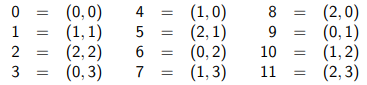
\includegraphics[scale=0.7]{numbers}
	\end{center}
	\item To perform arithmetic with large numbers, choose the moduli $m_1,...,m_n$ so that $m=m_1\cdots m_n>$ the result of the operations you want to carry out
	\item Then arithmetic can be performed with representations of numbers
	\item Example: compute $2\cdot 5$. Instead, multiply (2,2) and (2,1) component wise. 1st component modulo 3 and 2nd modulo 4. Get (1,2) which represents 10
	\item Advantages: can work with very large numbers and can compute in parallel
	\item Particularly good choices for $m_i$: numbers of the form $2^p-1$
\end{itemize} 
\section{Fermat's Little theorem}
\subsection{Theorem}
If p is a prime and a is not a multiple of p then $a^{p-1}\equiv 1 (\bmod p)$\\
Furthermore, for every integer a, $a^p\equiv a (\bmod p)$
\subsection{Example}
\begin{itemize}
	\item We know how to find inverses modulo prime p (via Euclid's algorithm)
	\item The above theorem gives an alternate approach: $a^{p-2}\cdot a\equiv 1 (\bmod p)$ hence $rem(a^{p-2},p)$ is the required inverse
\end{itemize}
Find the multiplicative inverse of 6 modulo 17\\
Solution: we need to compute $rem(6^{15},17)$, which can be done as follows.
$$\begin{aligned} 6 ^ { 2 } & \equiv 36 \equiv 2 ( \bmod 17 ) \\ 6 ^ { 4 } & \equiv \left( 6 ^ { 2 } \right) ^ { 2 } \equiv 2 ^ { 2 } \equiv 4 ( \bmod 17 ) \\ 6 ^ { 8 } & \equiv \left( 6 ^ { 4 } \right) ^ { 2 } \equiv 4 ^ { 2 } \equiv 16 ( \bmod 17 ) \\ 6 ^ { 15 } & \equiv 6 ^ { 8 } \cdot 6 ^ { 4 } \cdot 6 ^ { 2 } \cdot 6 \equiv 16 \cdot 4 \cdot 2 \cdot 6 \equiv 3 ( \bmod 17 ) \end{aligned}$$
Therefore, $rem(6^16,17)=3$ is the required inverse. Indeed $3\cdot 6\equiv 1 (\bmod 17)$
\section{Euler's theorem}
Recall Euler's $\phi$-function. $\phi(n)$ is the number of integers $1\leqslant a \leqslant n$ that are relatively prime with n.\\
Euler's theorem generalises Fermat's little theorem to non-prime moduli
\subsection{Theorem}
If n is a positive integer and $gcd(a,n)=1$ then $a^{\phi(n)}\equiv 1 (\bmod n)$
\subsection{Method}
\begin{itemize}
	\item If n is a prime then $\phi(n)=n-1$, so this is indeed a generalisation
	\item If gcd(a,n)=1, then, as we proved, the inverse of a modulo n exists and can be found using Euclid's algorithm
	\item By Euler's Theorem, it can also be found as $rem(a^{\phi(n)-1},n)$
	\item Can a have a multiplicative inverse modulo n is $gcd(a,n)>1$? No
	\begin{itemize}
		\item If the inverse $\overline{a}$ exists we have $\overline{a}a\equiv 1 (\bmod n)$, i.e. $\overline{a}a-1=kn$ for some k
		\item Rewrite as $\overline{a}a+(-k)n=1$, it follows that $gcd(a,n)=1$ 
	\end{itemize}
\end{itemize}
\section{Computing Euler's $\phi$-function}
\subsection{Lemma}
If $m_1$ and $m_2$ are relatively prime then $\phi(m_1\cdot m_2)=\phi(m_1)\cdot\phi(m_2)$.\\
If p is prime then $\phi(p^k)=p^k-p^{k-1}$
\subsection{Proof}
By the chinese remainder theorem, there is a 1 to 1 correspondence between
\begin{itemize}
	\item numbers x with $0\leqslant x < m_1m_2$ and
	\item pairs $(1_2,a_2)$ such that $0\leqslant a_i <m_i$ and $x\equiv a_i (\bmod m_i)$ for $i=1,2$
\end{itemize}
Since $a_i=rem(x,m_i)$ we have $gcd(x,m_i)=gcd(a_i,m_i)$ for i=1,2\\
We have $gcd(x,m_1,m_2)=gcd(x,m_1)\cdot gcd (x,m_2)=gcd(a_1,m_1)\cdot gcd(a_2,m_2) $ (the first equality holds because $gcd(m_1,m_2)=1$)\\
In particular, $gcd(x,m_1m_2)=1$ iff $gcd(a_1,m_1)=gcd(a_2,m_2)=1$. This immediately implies $\phi(m_1cdot m_2)=\phi(m_1)\cdot\phi(m_2)$
\subsection{Example}
$$\phi ( 75 ) = \phi \left( 3 \cdot 5 ^ { 2 } \right) = \phi ( 3 ) \cdot \phi \left( 5 ^ { 2 } \right) = \left( 3 ^ { 1 } - 3 ^ { 0 } \right) \cdot \left( 5 ^ { 2 } - 5 \right) = 40$$
\end{document}